\newpage
\section{Pembuatan Sistem Face Recognition}
Prose pertama untuk melakukan pengenalan wajah yaitu dengan mengumpulkan dataset yang akan di \emph{training} dengan menangkap citra wajah pada saat awal deteksi wajah yang akan 
disimpan dan dikumpulkan berdasarkan id yang telah dimasukkan user. Setelah dataset terkumpul, selanjutnya sistem akan melakukan \emph{training data} untuk mengenali wajah berdasarkan id. 
Kemudian proses penenalan wajah pun dilakukan dengan mendeteksi wajah mengunakan algoritma Haar-cascade classifier, lalu sistem akan melakukan pencocokan dengan menggunakan fitur LBPH 
untuk mencocokan wajah yang terdeteksi dengan dataset yang sudah di\emph{training} sebelumnya.
\begin{enumerate}[1.]
\item Proses mengumpulkan dataset dengan

- Memasukan library openCV, yaitu \textbf{cv2}
\begin{figure}[h!]
    \centering
    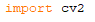
\includegraphics[width=0.3\linewidth]{images/fr_1.PNG}
    \caption{Memasukan library openCV}
\end{figure}

-  Proses face detection, untuk melakukan proses deteksi wajah akan menggunakan algoritma \emph{haarcascade}. Dengan fungsi \textbf{cv2.CascadeClassifier} pada baris pertama, 
pada baris kedua merupakan fungsi openCV untuk memasukan video atau kamera yang terhubung dengan \textbf{cv2.VideoCapture()}
\begin{figure}[h!]
    \centering
    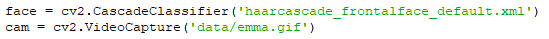
\includegraphics[width=0.85\linewidth]{images/fr_2.PNG}
    \caption{Proses face detection}
\end{figure}

- Menambahkan variabel 'jumlah' yang dimulai dari 0 untuk menyimpan data perulangan pengambilan gambar dataset
dan juga pada baris selanjutnya ada variabel 'id' wadah masukan user untuk id dataset
\begin{figure}[h!]
    \centering
    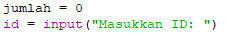
\includegraphics[width=0.5\linewidth]{images/fr_3.PNG}
    \caption{Tambah variabel}
\end{figure}
\newpage
- Membaca video atau kamera yang sudah dimasukkan sebelumnya dengan fungsi \textbf{read()}, dan untuk mengubah warna citra menjasi hitam-putih/grayscale
dengan fungsi \textbf{cv2.cvtColor}
\begin{figure}[h!]
    \centering
    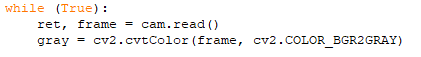
\includegraphics[width=0.85\linewidth]{images/fr_4.PNG}
    \caption{Membaca video dan merubah warna citra}
\end{figure}

- Pada baris pertama fungsi untuk deteksi wajah dengan fungsi \textbf{detectMultiScale()}. 
Pada baris selanjutnya ada fungsi membuat bingkai \textbf{cv2.rectangle} lalu ada pengulangan untuk jumlah gambar yang ditangkat
, lalu ada \textbf{cv2.imwrite} untuk menyimpan gambar data direktori dataset yang telah ditentukan, da \textbf{cv2.imshow} untuk 
menampilkan video atau kamera yang aka dideteksi dan diambil gambar untuk dataset.
\begin{figure}[h!]
    \centering
    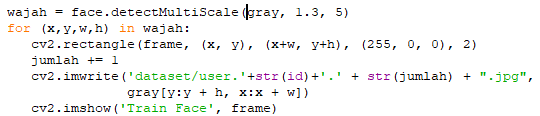
\includegraphics[width=0.85\linewidth]{images/fr_5.PNG}
    \caption{Penyimpanan dataset}
\end{figure}

- Menentukan jumlah gambar yang akan tersimpan pada dataset
\begin{figure}[h!]
    \centering
    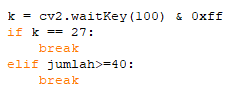
\includegraphics[width=0.5\linewidth]{images/fr_6.PNG}
    \caption{Mengatur jumlah gambar yang diambil}
\end{figure}
\newpage
- Keseluruhan kode program untuk pengambilan dataset
\begin{figure}[h!]
    \centering
    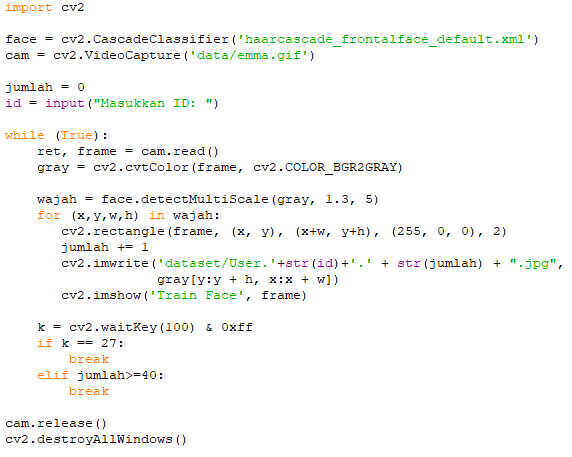
\includegraphics[width=0.85\linewidth]{images/fr_full.PNG}
    \caption{Kode pengambilan dataset}
\end{figure}

- Percobaan pengambilan dataset untuk tiga ID menggunakan masukan video
\begin{figure}[h!]
    \centering
    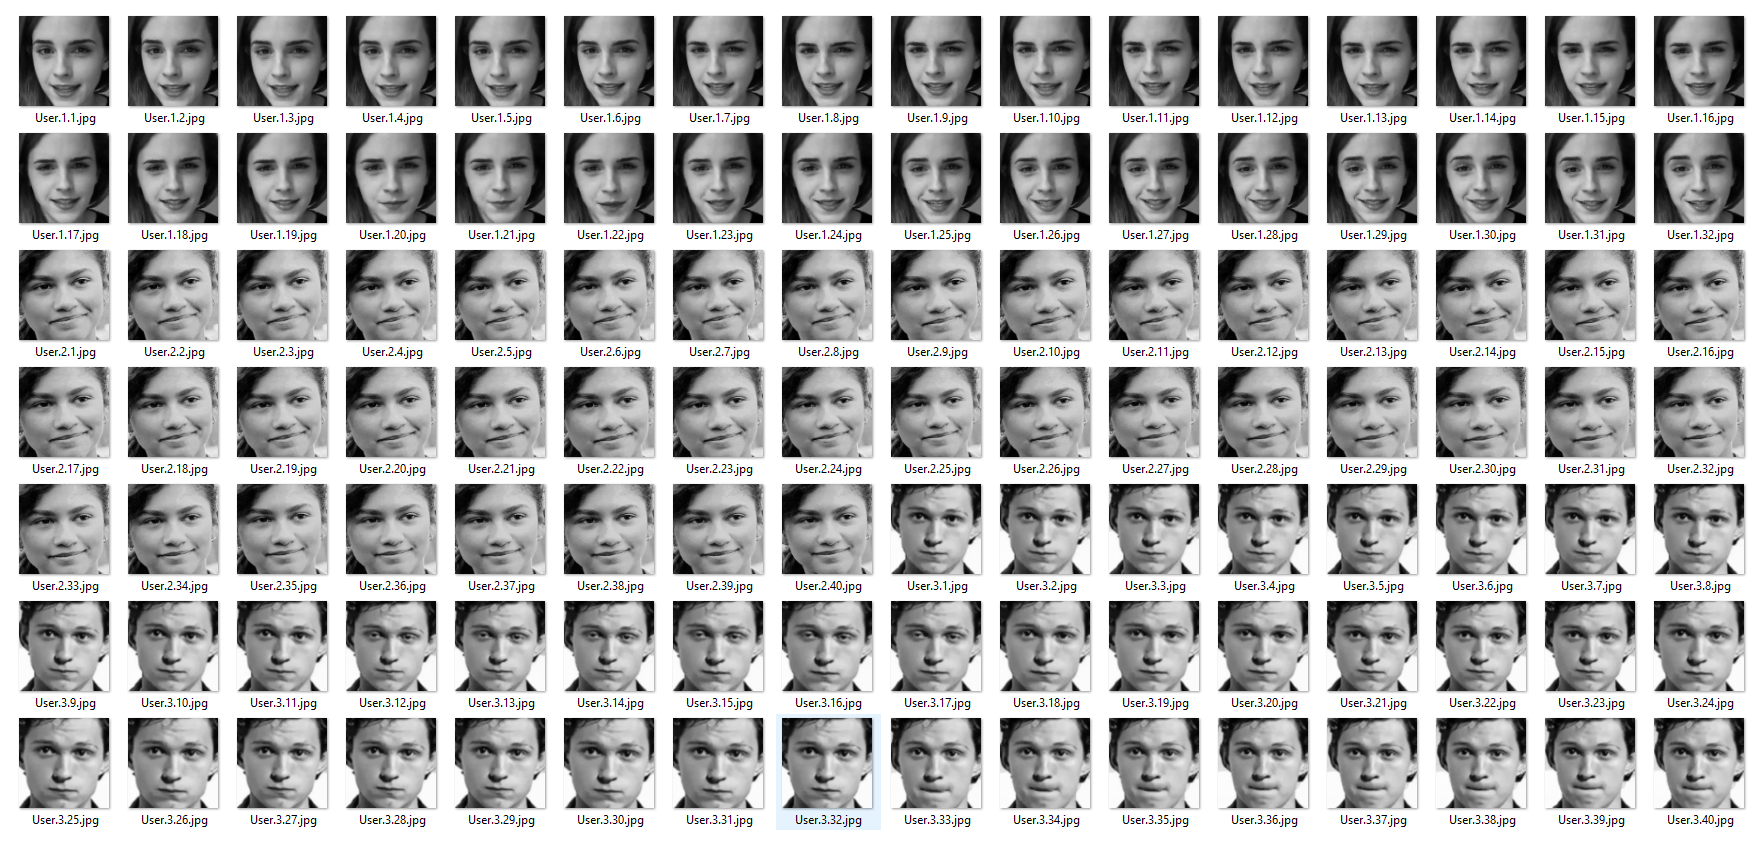
\includegraphics[width=1.2\linewidth]{images/dataset.PNG}
    \caption{Pengambilan dataset}
\end{figure}

\item Proses training dataset

- Import library cv2, numpy, Image from PIL (Pillow) library, dan os
\begin{figure}[h!]
    \centering
    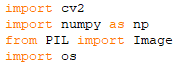
\includegraphics[width=0.4\linewidth]{images/train_1.PNG}
    \caption{Pengambilan dataset}
\end{figure}

- pada baris ke-1, memasukan nama direktori dataset pada variabel path 

Pada baris ke-2, untuk pengenalan wajah, menggunakan model algoritma LBPH yang sudah tersedia pada openCV

Pada bari ke-3,  Proses face detection, untuk melakukan proses deteksi wajah akan menggunakan algoritma haarcascade
\begin{figure}[h!]
    \centering
    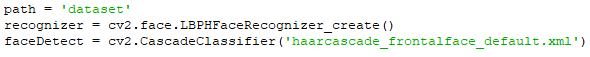
\includegraphics[width=0.9\linewidth]{images/train_2.PNG}
    \caption{Pengambilan dataset}
\end{figure}

- Membuat method atau fungsi untuk mendapatkan image dataset sebagai data training agar dikenali oleh bahasa komputer
\begin{figure}[h!]
    \centering
    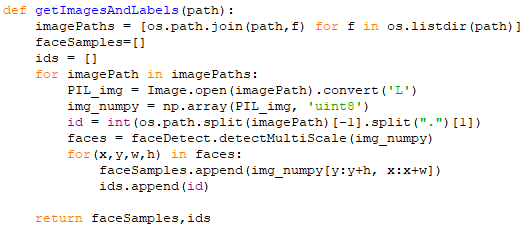
\includegraphics[width=0.9\linewidth]{images/train_3.PNG}
    \caption{Pengambilan dataset}
\end{figure}\\
Memasukan direktori dataset pada variabel path menggunakan \textbf{os.path.join()} kedalam variabel imagePath.
Lalu kumpulan image training akan diubah menggunakan library PIL menjadi sebuah array. Setelah itu, array data training akan dibuat oleh numpy.
Dimana array yang diambil merupakan id dan juga faceSample.
\newpage
- Training data
\begin{figure}[h!]
    \centering
    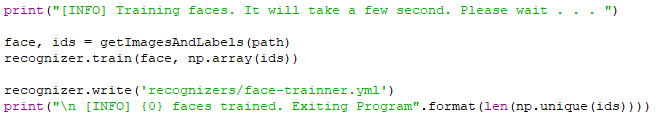
\includegraphics[width=0.9\linewidth]{images/train_4.PNG}
    \caption{Pengambilan dataset}
\end{figure}\\
Fungsi "getImagesAndLabels (path)", akan mengambil semua foto di direktori: "dataset/", mengembalikan 2 array: "Ids" dan "faces". 
Dengan array tersebut sebagai input, data akan di training menggunakan fungsi \textbf{recognizer.train()}
Untuk hasil training data akan disimpan dalam bentuk \textbf{.yml} pada direktori recognizers dengan fungsi \textbf{recognizer.write()}

- Proses training data
\begin{figure}[h!]
    \centering
    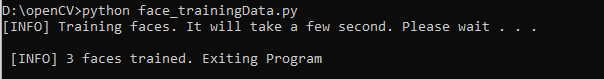
\includegraphics[width=0.9\linewidth]{images/train_data.PNG}
    \caption{Pengambilan dataset}
\end{figure}

- Hasil training data berbentuk file \textbf{.yml}
\begin{figure}[h!]
    \centering
    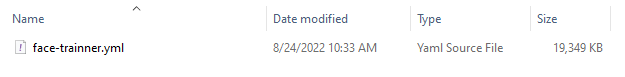
\includegraphics[width=1\linewidth]{images/hasil_train.PNG}
    \caption{Pengambilan dataset}
\end{figure}

\item Proses pengenalan wajah
\end{enumerate}
